\documentclass[a4paper,12pt]{book}

% Paquetes necesarios
\usepackage[utf8]{inputenc}   % Codificación de caracteres
\usepackage[spanish]{babel}   % Idioma español
\usepackage[T1]{fontenc}      % Codificación de fuentes
\usepackage{amsmath, amssymb} % Símbolos matemáticos
\usepackage{graphicx}         % Inclusión de gráficos
\usepackage{cite}             % Gestión de citas
\usepackage{hyperref}         % Enlaces y referencias
\usepackage{geometry}         % Configuración de márgenes
\usepackage{fancyhdr}         % Encabezados y pies de página
\usepackage{titlesec}         % Formato de títulos
\usepackage{booktabs}         % Tablas profesionales
\usepackage{caption}          % Personalización de leyendas
\usepackage{enumitem}         % Personalización de listas
\usepackage{float}
\usepackage{tcolorbox}
\usepackage[table]{xcolor} % Paquete para colores en tablas
\usepackage{colortbl}       % Complemento para colorear celdas específicas
\usepackage{multirow}       % Combinar celdas en tablas
\usepackage{makecell}       % Combinar celdas en tablas
\usepackage{enumitem}
\usepackage{amsmath}
\usepackage{eurosym}
\usepackage{tikz}
\usepackage{listings}
\usepackage{color}
\usepackage{float}
\usepackage{pdfpages}
\usepackage{subfigure}
\usepackage{pgffor}

% Configuración de márgenes
\geometry{left=3cm, right=3cm, top=2.5cm, bottom=2.5cm}

% Configuración de encabezados y pies de página
% \setlength{\headheight}{14.49998pt}
\pagestyle{fancy}
\fancyhf{}
\fancyhead[L]{Universidad de Granada}
\fancyhead[L]{\nouppercase{\leftmark}}

% \fancyhead[C]{Escuela Técnica Superior de Ingenierías Informática}
\fancyhead[R]{Fundamentos de Base de Datos}
\fancyfoot[L]{\rule[0pt]{\textwidth}{0.2pt}\\Ismael Sallami Moreno}
\fancyfoot[C]{\rule[0pt]{\textwidth}{0.2pt}\\\thepage}
\fancyfoot[R]{\rule[0pt]{\textwidth}{0.2pt}\\\today}
\renewcommand{\sectionmark}[1]{\markboth{#1}{}} % Configura \leftmark para que solo muestre la sección


% Formato de títulos
\titleformat{\section}{\large\bfseries}{\thesection.}{0.5em}{}
\titleformat{\subsection}{\normalsize\bfseries}{\thesubsection.}{0.5em}{}

% Datos del documento
\title{\textbf{Temario Inteligencia Artificial}}
\author{
    Ismael Sallami Moreno \\
    \texttt{ism350zsallami@correo.ugr.es}
}
\date{
    \vspace{1cm}
    \begin{tabular}{rl}
        \textbf{Asignatura:} & Fundamentos de Base de Datos \\
        \textbf{Tema:} & Teoría \\
        \textbf{Fecha:} & \today
    \end{tabular}
}

% Comando para definir código en línea que se muestra en cursiva y no se sale del PDF
\newcommand{\inlinecode}[1]{\texttt{\textit{#1}}}


\begin{document}

% Portada
\begin{titlepage}
    \begin{center}
        % \vspace*{1cm}
        
        % \Huge
        % \textbf{Práctica Contabilidad Financiera II}
        \Huge \textbf{FBD - Relación de Ejercicios S1 y S2: Modelo Entidad-Relación y Paso a Tablas} 
        % \vspace{0.5cm}
        % \LARGE
        % \textbf{Ismael Sallami Moreno}\\
        % \LARGE
        % \texttt{ism350zsallami@correo.ugr.es}
        % \LARGE
        % \url{https://github.com/Ismael-Sallami}
        
        % \vfill
        
        % \Large
        % \textbf{Universidad de Granada}
        
        \vspace{0.8cm}
        
        \begin{tikzpicture}[remember picture, overlay]
            \node[opacity=0.2] at (current page.center) {
\includegraphics[width=\paperwidth,height=\paperheight]{portada.jpg}};
            \node[align=center] at (current page.center) {
                
                \vspace{0.5cm}
                \LARGE \textbf{Ismael Sallami Moreno} \\
                \LARGE \texttt{ism350zsallami@correo.ugr.es} \\
                %\LARGE \url{https://ismael-sallami.github.io/} \\
                %\LARGE \url{https://elblogdeismael.github.io/} \\
                \vspace{2cm}
                \Large \textbf{Universidad de Granada} \\
                \vspace{0.8cm}
                % \Large \textbf{2025}
            };
        \end{tikzpicture}
        \vfill
        
        \Large
        \textbf{2025}
        
    \end{center}
\end{titlepage}
\newpage


%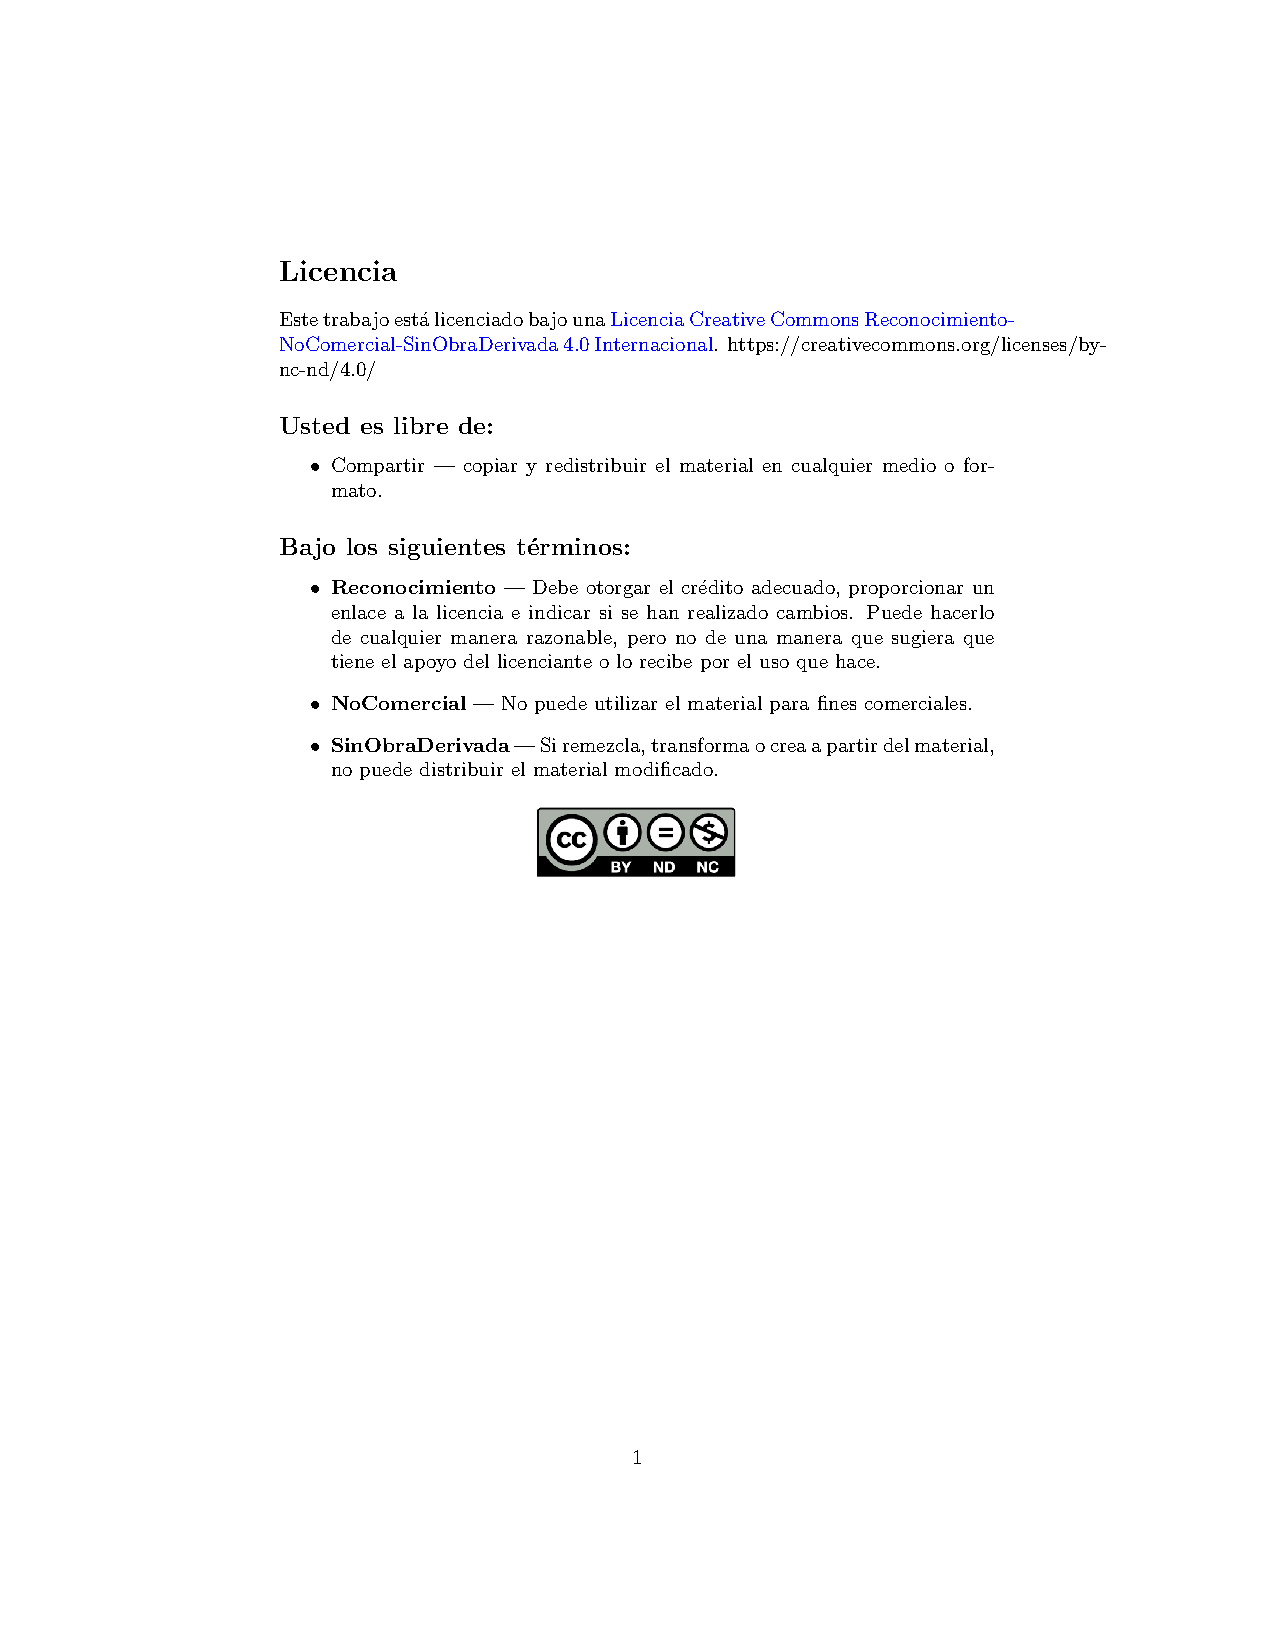
\includepdf[pages=-]{../../../../licencia.pdf}
% Tabla de contenidos
\tableofcontents
\newpage

\chapter{Modelo Entidad-Relación y Paso a Tablas}
\newpage
\section{Ejercicios de la Relación S1 y S2}
\foreach \imagen in {
    images/EjercicioS1S2/EjerciciosS1S2/Ejercicios1P1.png,
    images/EjercicioS1S2/EjerciciosS1S2/Ejercicios1P2.png,
    images/EjercicioS1S2/EjerciciosS1S2/Ejercicios1P3.png,
    images/EjercicioS1S2/EjerciciosS1S2/Ejercicios1P4.png,
    images/EjercicioS1S2/EjerciciosS1S2/Ejercicios1P5.png,
    images/EjercicioS1S2/EjerciciosS1S2/Ejercicios1P6.png,
    images/EjercicioS1S2/EjerciciosS1S2/Ejercicios1P7.png,
    images/EjercicioS1S2/EjerciciosS1S2/Ejercicios1P8.png,
    images/EjercicioS1S2/EjerciciosS1S2/Ejercicios1P9.png,
    images/EjercicioS1S2/EjerciciosS1S2/Ejercicios1P10.png,
    images/EjercicioS1S2/EjerciciosS1S2/Ejercicios1P11.png,
    images/EjercicioS1S2/EjerciciosS1S2/Ejercicios1P12.png,
    images/EjercicioS1S2/EjerciciosS1S2/Ejercicios1P13.png,
    images/EjercicioS1S2/EjerciciosS1S2/Ejercicios1P14.png,
    images/EjercicioS1S2/EjerciciosS1S2/Ejercicios1P15.png,
    images/EjercicioS1S2/EjerciciosS1S2/Ejercicios1P16.png,
    images/EjercicioS1S2/EjerciciosS1S2/Ejercicios1P17.png,
    images/EjercicioS1S2/EjerciciosS1S2/Ejercicios1P18.png,
    images/EjercicioS1S2/EjerciciosS1S2/Ejercicios1P19.png,
    images/EjercicioS1S2/EjerciciosS1S2/Ejercicios1P20.png,
    images/EjercicioS1S2/EjerciciosS1S2/Ejercicios1P21.png,
    images/EjercicioS1S2/EjerciciosS1S2/Ejercicios1P22.png,
    images/EjercicioS1S2/EjerciciosS1S2/Ejercicios1P23.png,
    images/EjercicioS1S2/EjerciciosS1S2/Ejercicios1P24.png,
    images/EjercicioS1S2/EjerciciosS1S2/Ejercicios1P25.png,
    images/EjercicioS1S2/EjerciciosS1S2/Ejercicios1P26.png,
    images/EjercicioS1S2/EjerciciosS1S2/Ejercicios1P27.png,
    images/EjercicioS1S2/EjerciciosS1S2/Ejercicios1P28.png,
    images/EjercicioS1S2/EjerciciosS1S2/Ejercicios1P29.png,
    images/EjercicioS1S2/EjerciciosS1S2/Ejercicios1P30.png
} {
    \begin{figure}[H]
        \centering
        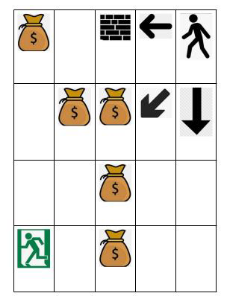
\includegraphics[width=\textwidth]{\imagen}
        %\caption{Ejercicio correspondiente a \imagen}
    \end{figure}
}





\newpage
% Referencias
\begin{thebibliography}{99}
\bibitem{Referencia1}
Ismael Sallami Moreno, \textbf{Estudiante del Doble Grado en Ingeniería Informática + ADE}, Universidad de Granada, 2025.
% \bibitem{Referencia2}
% Autor(es), \emph{Título del libro}, Editorial, año.

% \bibitem{Referencia3}
% Autor(es), \emph{Título del documento}, Nombre de la Conferencia, páginas, año.
\end{thebibliography}

\end{document}
